\documentclass[11pt,letterpaper,titlepage]{article}

\usepackage{geometry}
\geometry{left=1.5cm,right=1.5cm,top=1.5cm,bottom=2.5cm}

\usepackage{setspace}
\onehalfspacing

\usepackage{fancyhdr}

\usepackage{amsmath}
\DeclareMathOperator*{\argmax}{arg\,max}
\DeclareMathOperator*{\argmin}{arg\,min}
\renewcommand{\vec}[1]{\mathbf{#1}}

\usepackage{amssymb}

\usepackage{booktabs}

\usepackage{pifont}

\usepackage{hyperref}
\hypersetup{
    colorlinks,
    citecolor=black,
    filecolor=black,
    linkcolor=black,
    urlcolor=black
}

\usepackage{trace}

\usepackage{tikz}

\pagestyle{fancy}
\lhead{}
\rhead{}
\lfoot{ECEN 662 Estimation and Detection Theory}
\cfoot{\thepage}
\rfoot{Notes @Lei Wang}
\renewcommand{\headrulewidth}{0pt}
\renewcommand{\headwidth}{\textwidth}
\renewcommand{\footrulewidth}{0.4pt}
\newcommand{\RomanNumeralCaps}[1]
    {\MakeUppercase{\romannumeral #1}}
    
\begin{document}

\begin{titlepage}
  \centering
	{\scshape\large Texas A\&M University \par}
	\vspace{1cm}
	{\scshape\Large Department of Electrical and Computer Engineering \par}
	\vspace{4cm}
    \vspace{0.5cm}
	{\huge\bfseries ECEN 662 Estimation and Detection Theory\par}
	\vspace{4cm}
	{\Large Notes\par}
	\vspace{1cm}
	{\Large Student: Lei Wang (Wilson)\par}
	\vspace{1cm}
	{\Large UIN: 829009485\par}
	\vspace{1cm}
	{\Large Instructor: Dr. Jean-Francois Chamberland\par}
	\vspace{4cm}
	\vfill

  % Bottom of the page
% 	{\large Submitted: February 11th, 2020 \par}

\end{titlepage}

\newpage

\tableofcontents{}

\newpage

\section{Lesson 1 1.14.2020}

Statistical inference.

\subsection{Probability Laws:}

\begin{enumerate}

    \item Non-negative
    
    \item Normalization: sum to 1
    
    \item Countable additivity: if disjoint, $Pr(\sum N)=\sum Pr(N)$
    
\end{enumerate}

\subsection{Sample Space:}

A sample space $\Omega$ contains the outcomes $\omega$, which are disjoint, mutually exclusive and collectively exhaustive.

A collection of subsets of $S$ is called a sigma algebra $B$ if it satisfies the 3 properties:

\begin{enumerate}

    \item $\phi \in B$
    
    \item If $A \in B$, then $A^C \in B$
    
    \item If $A_1, A_2... \in B$, then $\bigcup\limits_{i=1}^{\infty} \in B$ (closed under countable unions)
    
\end{enumerate}

From Wikipedia: In mathematical analysis and in probability theory, a $\sigma$-algebra (also $\sigma$-field) on a set $X$ is a collection $\sum$ of subsets of $X$ that includes $X$ itself, is closed under complement, and is closed under countable unions.

\newpage

\section{Lesson 2 1.16.2020}

\subsection{Conditional Probability:}

\begin{equation*}
    Pr(A|B) = \frac{Pr(A\cap B)}{Pr(B)} \in [0, 1] \text{, } Pr(A\cap B) \in [0, Pr(B)] \text{, } Pr(B) > 0
\end{equation*}

\begin{itemize}

    \item Restriction to the sample space
    
    \item $Pr(.|B)$: new probability laws, still need to satisfy the 3 axioms
    
    \item $Pr(B) = \sum Pr(B|A_i)Pr(A_i)$
    
\end{itemize}

\subsection{Countable Additivity:}

Disjoint $A_1$, $A_2$, $A_3$...

\begin{equation*}
    \begin{aligned}
        Pr(\bigcup\limits_{i=1}^{\infty} A_i) &= \sum_{i=1}^{\infty} Pr(A_i) \\
        Pr(\{\bigcup\limits_{i=1}^{\infty} A_i\}|B) &= \frac{Pr(\{\bigcup\limits_{i=1}^{\infty} A_i \}\cap B)}{Pr(B)} \text{, the numerator distributes the set over the union} \\
        &= \frac{Pr(\bigcup\limits_{i=1}^{\infty} \{A_i \cap B\})}{Pr(B)} \\
        &= \frac{\sum\limits_{i=1}^{\infty} Pr(A_i \cap B)}{Pr(B)} \\
        &= \sum\limits_{i=1}^{\infty} Pr(A_i | B) \\
    \end{aligned}
\end{equation*}

\subsection{Independence:}

\begin{itemize}

    \item $Pr(A \cap B) = Pr(A) Pr(B)$
    
    \item $Pr(A|B) = \frac{Pr(A \cap B)}{Pr(B)} = \frac{Pr(A)Pr(B)}{Pr(B)} = Pr(A)$, if independent and $Pr(B) > 0$
    
    \item $Pr(B|A) = Pr(B)$ if independent and $Pr(A) > 0$
    
\end{itemize}

\newpage

\section{Lesson 3 1.21.2020}

\subsection{Event Independence:}

\begin{itemize}

    \item $Pr(A_1 \cap A_2 \cap A_3) = Pr(A_1)Pr(A_2)Pr(A_3)$
    
    \item Also check each pair
    
    \item 3 sets, 4 conditions to check
    
    \item $k$ sets: $2^k - k -1$ conditions to check
    
    \item Why pairwise independence is not enough? i.e. throwing a coin twice
    
\end{itemize}

\subsection{Random Variable:}

\begin{itemize}

    \item $X: \Omega \rightarrow \mathbb{R}$, sample space to real numbers
    
    \item Induced probability law: $P_X(x \in A), A \subset \mathbb{R}$, $X^{-1} (A) \subset \Omega$:
    
    $P_X(x \in A) = Pr(x^{-1} (A))$, $x^{-1} (A)$ is the event
    
\end{itemize}

\subsection{CDF:}

\begin{itemize}

    \item $F_X (x) = Pr(X \leq x)$
    
    \item Discrete: PMF, steps, right-continuous
    
    \item Continuous: PDF, $F_X (x) = \int_{-\infty}^{x} f_X(t)dt$
    
    \item Mixed
    
\end{itemize}

\newpage

\section{Lesson 4 1.23.2020}

\subsection{Transformation:}

\begin{itemize}

    \item $Y = g(X) = g \circ X$: composition of functions
    
    $Y$ is a random variable
    
    $Pr(Y \in A)$
    
    $Y = g \circ X \rightarrow Pr(g(X) \in A) = Pr(x \in g^{-1}(A))$: $g^{-1}(A) \rightarrow$ event under $P_X$, the pre-image of $A$ under $g$
    
    \item Suupose $G$ is strictly increasing and continuous. How to you relate $f_Y(.)$ to $f_X(.)$?
    
    \begin{equation*}
        \begin{aligned}
            Pr(Y \leq y) &= Pr(x \in g^{-1}((-\infty, y])) \\
            &= Pr(x \in (-\infty, g^{-1} (y)]) \\
            &= F_X(g^{-1} (y))
        \end{aligned}
    \end{equation*}
    
    \begin{equation*}
        \begin{aligned}
            \frac{d}{dy} F_Y(y) &= \frac{d}{dy} F_X (g^{-1}(y)) \\
            &= f_X(g^{-1}(y)) \cdot \frac{d}{dy} g^{-1} (y) \\
            &= f_Y(y)
        \end{aligned}
    \end{equation*}
    
    \item What if $y$ is strictly decreasing and continuous?
    
    \begin{equation*}
        \begin{aligned}
            Pr(Y \leq y) &= Pr(x > g^{-1}(y)) \\
            &= 1 - F_X(g^{-1}(y)) \\
            f_Y(y) &= f_X(g^{-1}(y)) \cdot (- \frac{d}{dy} g^{-1}(y))
        \end{aligned}
    \end{equation*}
    
    Can use an absolute value sign here
    
    \item In general, for strictly increasing or decreasing functions:
    
    \begin{equation*}
        \begin{aligned}
            f_Y (y) &= f_X (g^{-1}(y))|\frac{d}{dy} g^{-1}(y)| \text{ on support} \\
            &= 0 \text{, if out of support}
        \end{aligned}
    \end{equation*}
    
    \item 
    
    \begin{equation*}
        \begin{aligned}
            Pr(Y \leq y) &= Pr(F_X(x) \leq y) \\
            &= Pr(x \in F^{-1}_X(y)) \\
            &= Pr(x \leq F^{-1}_X(y)) \text{, because } F_X \text{ is increasing, CDF} \\
            &= F_X(F^{-1}(y)) \\
            &= y \text{, provided } 0 \leq y \leq 1 \\
            F_Y(y) &= 1 \text{, if } y \in [0, 1] \\
            &= 0 \text{, otherwise, i.e. a uniform random variable}
        \end{aligned}
    \end{equation*}
    
\end{itemize}

\subsection{Uniform Random Variable:}

\begin{itemize}
    
    \item $Y=F_X(x)$ is uniform
    
    \item $U=F^{-1}_X(y)$
    
    \item Every continuous random variable can be obtained by taking a function of uniform random variable
    
    \item Use the uniform random variable to build other random variables
\end{itemize}

\newpage

\section{Lesson 5 1.28.2020}

\subsection{Condense Information:}

\begin{itemize}

    \item $f_X(x)dx$, can be made continuous to integers, i.e. PMF and CDF
    
    \item $X: f_X(.)$: expected return on investment and risk
    
    \item Expectation: $E[X]$, a function of the distribution of a random variable
    
    \begin{equation*}
        \begin{aligned}
            E[X] &= E(f_X(x)) \\
            &= \int_\mathbb{R} x f_X(x) dx
        \end{aligned}
    \end{equation*}
    
    The expectation does not always exist: Cauchy distribution has no expectation.
    
    \item Variance: $Var[X]$, a function of the distribution of random variable, also known as the second centralized moment
    
    \begin{equation*}
        \begin{aligned}
            Var[X] = \int_\mathbb{R} (x-\mu)^2 f_X(x)dx
        \end{aligned}
    \end{equation*}
    
    \item Standard deviation: $\sigma[X] = \sqrt{Var[X]}$
    
    \item $E[X^2]$ and $E[(X - E[X])^2]$ impose a $l_2$ structure or inner-product space
\end{itemize}

\subsection{argmin:}

\begin{itemize}
    \item 
    
    \begin{equation*}
        \begin{aligned}
            \argmin_C E[(X-C)^2]
        \end{aligned}
    \end{equation*}
    
    \item Take the derivative and set to 0
    
    \item Take the second derivative to check if it is min or not
    
    \item
    
    \begin{equation*}
        \begin{aligned}
            \argmin_c E[(X-c)^2] &= \argmin_c E[(X^2 - 2cX + c^2] \\
            &= \argmin_c E[X^2] - 2cE[X] + E[c^2] \\
        \end{aligned}
    \end{equation*}
    
    \item Decrease $E[X^2]$, increase $E[X]$: set both to 0
    
    \item
    
     \begin{equation*}
        \begin{aligned}
            \frac{d}{dc} \int (x-c)^2 f_X(x) dx &= \int \frac{\partial}{\partial c} (x-c)^2 f_X(x)dx \\
            &= \int -2(x-c) f_X(x) dx \\
            c &= E[X] \text{, after a second derivative test} \rightarrow min\\
        \end{aligned}
    \end{equation*}
    
    \item Limit not function of $c$, Lipschitz condition, fundmental theorem of calculus, dominated convergence theorem...
    
\end{itemize}

\subsection{Expectation, Moments and Moment Generating Function:}

\begin{itemize}

    \item $E[g(X)] = \int g(x) f_X(x) dx$
    
    \item $E[.]$ is a linear operator: $E[aX + b] = aE[X] + b$
    
    \item $E[X^n]$: moments
    
    \item $E[(X - \mu)^n]$: $n^{th}$ centralized moment
    
    \item $M_X(t) = E[e^{tX}]$: moment generating function
    
    \item The moment generating function does not always exist and exists if expectation exists in a neighbourhood of 0
    
    \item $X_1, X_2, X_3...$ such that the moments converge, still, the distribution may not be unique
    
    \item $M_{X_1}, M_{X_2}, M_{X_3}...$ such that they converge over the neighbourhood of 0, then the distribution is unique
    
    \item Moment generating function for general function: Laplace transform
    
    \item Characteristic equation: Fourier transform
    
\end{itemize}

\subsection{Contour Integral, Complex Analysis:}

\begin{itemize}

    \item $\oint$ in the complex plane to reverse a Laplace transform
    
\end{itemize}

\subsection{Gaussian Distribution:}

\begin{itemize}
    
    \item PDF, does not have a closed form indefinite integral:
    
    \begin{equation*}
        \begin{aligned}
            f_X(x) = \frac{1}{\sigma \sqrt{2\pi}} e^{-\frac{(x-\mu)^2}{2\sigma^2}} \text{, } x \in \mathbb{R}
        \end{aligned}
    \end{equation*}
    
    \item To find out where $\frac{1}{\sqrt{2\pi}}$ comes from:
    
    \begin{equation*}
        \begin{aligned}
            \int_{-\infty}^{\infty} \int_{-\infty}^{\infty} f_X(x) f_X(y) dx dy &= \int_{-\infty}^{\infty} \int_{-\infty}^{\infty} e^{-\frac{x^2}{2}} e^{-\frac{y^2}{2}} dx dy \\
            &= \int_{-\infty}^{\infty} \int_{-\infty}^{\infty} e^{-\frac{1}{2}(x^2 + y^2)} dx dy \text{, use polar coordnates}\\
            &= \int_{-\pi}^{\pi} \int_{0}^{\infty} r e^{-\frac{r^2}{2}} dr d\theta \\
            &= -e^{-\frac{r^2}{2}}\big|_{0}^{\infty} - \frac{1}{2} 2r e^{-\frac{r^2}{2}} \\
            &= 1
        \end{aligned}
    \end{equation*}
    
    \item Add $\frac{1}{\sqrt{2\pi}}$ to let the integral be 1
    
    \item $r$: the Jacobian, physical meaning is the contraction and the expansion of the space
    
    \item $Var[X] = \sigma^2$:
    
    \begin{equation*}
        \begin{aligned}
            Var[X] &=\int_{-\infty}^{\infty} (x - \mu)^2 \frac{1}{\sigma \sqrt{2\pi}} e^{-\frac{(x-\mu)^2}{2\sigma^2}} dx \text{, use integration by parts to solve} \\
            \int_{-\infty}^{\infty} \frac{1}{\sigma \sqrt{2\pi}} e^{-\frac{(x-\mu)^2}{2\sigma^2}} dx &= 1 \\
            \frac{d}{d\sigma} \int_{-\infty}^{\infty} e^{-\frac{(x-\mu)^2}{2\sigma^2}} dx &= \frac{d}{d\sigma} \sigma \sqrt{2\pi} \\
            \int_{-\infty}^{\infty} \frac{\partial}{\partial \sigma} e^{-\frac{(x-\mu)^2}{2\sigma^2}} dx &= \sqrt{2\pi} \\
            \int_{-\infty}^{\infty} e^{-\frac{(x-\mu)^2}{2\sigma^2}} \frac{(x-\mu)^2}{\sigma^3} dx &= \sqrt{2\pi} \\
            \int_{-\infty}^{\infty} \frac{(x-\mu)^2}{\sigma\sqrt{2\pi}} e^{-\frac{(x-\mu)^2}{2\sigma^2}} dx &= \sigma^2
        \end{aligned}
    \end{equation*}
    
\end{itemize}

\subsection{Inequalities:}

\begin{itemize}

    \item Expection on functions:
    
    \begin{equation*}
        \begin{aligned}
            g(x) &\leq h(x) \\
            \int_{a}^{b} g(x) dx &\leq \int_{a}^{b} h(x) dx \\
            f_X(x) g(x) &\leq f_X(x) h(x) \text{, therefore} \\
            \int f_X(x) g(x) dx &\leq \int f_X(x) h(x) dx \\
            E[g(x)] &\leq E[h(x)]
        \end{aligned}
    \end{equation*}

    \item Indicator function:
    
    \begin{equation*}
        \begin{aligned}
            Pr(x \geq a) &= E[\mathbb{I}_{[a, \infty]}(x)], x \geq 0 \\
            Pr(x \geq a) &\leq \frac{1}{a} E[X] \text{, Markov Inequality}
        \end{aligned}
    \end{equation*}

\end{itemize}

\newpage

\section{Lesson 6 1.30.2020}

\subsection{Multi-Variable Random Variables:}

\begin{itemize}

    \item Joint cumulative function: consider the two-variable scenario
    
    \begin{equation*}
        \begin{aligned}
            F_{X, Y}(x, y) &= Pr(X \leq x, Y \leq y) \\
            &= Pr(\{\omega \in \Omega: X(\omega) \leq x, Y(\omega) \leq y\})
        \end{aligned}
    \end{equation*}
    
    \item Marginal distribution: 
    
    \begin{equation*}
        \begin{aligned}
            \lim_{y \to \infty} F_{X, Y} (x, y) &= F_X(x) \\
            \lim_{x \to -\infty} F_{X, Y} (x, y) &= 0
        \end{aligned}
    \end{equation*}
    
    \item Joint PDF:
    
    \begin{equation*}
        \begin{aligned}
            f_{X, Y}(x, y) &= \frac{\partial^2}{\partial x \partial y} F_{X, Y}(x, y) \\
            \int_\mathbb{R} \int_\mathbb{R} f_{X, Y}(x, y) dx dy &= 1
        \end{aligned}
    \end{equation*}
    
\end{itemize}

\subsection{Indicator Function:}

\begin{equation*}
    \begin{aligned}
        Pr(A) &= \int_A f_X(x) dx \\
        &= \int_\mathbb{R} \mathbb{I}_{A(x)} f_X(d) dx
    \end{aligned}
\end{equation*}

\subsection{Conditional Probability:}

\begin{itemize}

    \item PDF: given event $A$
    
    \begin{equation*}
         F_X|A(x) =\frac{Pr(\{X \leq x\} \cap A)}{Pr(A)}
    \end{equation*}
    
    \item CDF:
    
    \begin{equation*}
        f_{X|A}(x) = \frac{\partial}{\partial x} F_{X|A}(x)
    \end{equation*}
    
    \item Conditioning on a value: $X$, $Y$ are continuous random variables
    
    \begin{equation*}
        f_{X|Y}(x|y) = \frac{f_{X, Y}(x, y)}{f_Y(y)}
    \end{equation*}
    
    Cannot get this from the definition of probabilities:
    
    
    \begin{equation*}
        \begin{aligned}
            Pr(x \leq X \leq x + \Delta x, y \leq Y \leq y + \Delta y) \text{, } X, Y \text{ have non-vanishing probability} \\
        \end{aligned}
    \end{equation*}
    
    Therefore,
    
    \begin{equation*}
        \begin{aligned}
            f_{X|Y}(x|y) &= \frac{Pr(x \leq X \leq x + \Delta x, y \leq Y \leq y + \Delta y)}{Pr(y \leq Y \leq y + \Delta y)} \text{, using the Riemann approach} \\
            &\approx \frac{f_{X, Y}(x, y) \Delta x \Delta y}{f_Y(y) \Delta y} \text{, joint PDF needs to be smooth enough} \\
            &= f_{X|Y}(x|y) dx
        \end{aligned}
    \end{equation*}
    
    Suppose $f_X(x)$, $u = g(x)$, $g(x)$ being strictly increasing and differentiable,
    
    \begin{equation*}
        \begin{aligned}
            f_U(u) &= f_X(g^{-1}(u)) \cdot |g'(x)| \\
            f_X(x) dx &\rightarrow f_U(x) \frac{dx}{du} \cdot du
        \end{aligned}
    \end{equation*}
    
\end{itemize}

\subsection{Joint Gaussian Distribution:}

\begin{itemize}

    \item PDF

    \begin{equation*}
        \begin{aligned}
            f_{X, Y}(x, y) &= \frac{1}{2 \pi} e^{-\frac{1}{2} (x^2 + y^2)} \\
            f_{\vec{X}, \vec{Y}}(\vec{x}, \vec{y}) &= \frac{1}{2 \pi |\Sigma|} e^{-\frac{1}{2}(\vec{x} - \vec{y})^{T} \Sigma^{-1}(\vec{x} - \vec{y})}
        \end{aligned}
    \end{equation*}
    
    \item Gaussian vectors: $ \vec{X} = [x_1, x_2, x_3...]$, $E[\vec{X}]$, $E[(\vec{X} - E[\vec{X}])(\vec{X} - E[\vec{X}])^T]$
    
    \begin{equation*}
        \begin{aligned}
            f_{\vec{X}}(\vec{x}) &= \frac{1}{(2 \pi)^{\frac{n}{2}} |\Sigma|^{\frac{1}{2}}} e^{-\frac{1}{2} (\vec{x} - E[\vec{X}])^{T} \Sigma^{-1}(\vec{x} - E[\vec{X}])}
        \end{aligned}
    \end{equation*}
    
    \item $Y = X + N$: $X$, $N$ Gaussian and independent
    
    \begin{equation*}
        \begin{aligned}
            f_{X, Y}(x, y) &= \frac{1}{2 \pi \sigma_x \sigma_y} e^{-\frac{1}{2} (x^2 = y^2)} \\
            E[Y] &= 0 \\
            E[Y^2] &= E[(X + N)^2] \\
            &= E[X^2 + N^2 + 2X N] \\
            &= 1 + 1 + 2 E[X N] \\
            &= 2 \\
            Var[Y] &= 2 - 0 \\
            &= 2
        \end{aligned}
    \end{equation*}
    
    \item Joint Gaussian: marginalize $\rightarrow$ Gaussian
    
    \item Joint Gaussian: conditional $\rightarrow$ Gaussian
    
\end{itemize}

\newpage

\section{Lesson 7 2.4.2020}

\subsection{Linear Regression:}

\begin{itemize}

    \item A number of data points: hope to draw a line of best fit
    
    \item To do so, need to minimize the distance between the output and the data $\rightarrow$ or the square of the distance
    
\end{itemize}

\subsection{Convex Function:}

\begin{itemize}
    
    \item Inverse: expensive, not always feasible
    
    \item Use an iterative approach, i.e. gradient descent, but may step over the optimal
    
\end{itemize}

\subsection{Loss Function:}

\begin{itemize}
    
    \item Measure on how well the prediction is: $y - \hat{y}$ (real - predict)
    
    \item Make the loss function convex: $(y - \hat{y}^2)$
    
    \item Mean square error: $y_i$ is the observation, does not depend on anything
    
    \begin{equation*}
        \begin{aligned}
            \frac{1}{n} \sum_{i=1}^{n} (y_i - \hat{y_i})^2 = \frac{1}{n} \sum_{i=1}^{n} (y_i - (\beta_1 x_i + \beta_0))^2
        \end{aligned}
    \end{equation*}
    
    To minimize the mean square error:
    
    \begin{equation*}
        \begin{aligned}
            \frac{\partial}{\partial \beta_1} \frac{1}{n} \sum_{i=1}^{n} (y_i - (\beta_1 x_i + \beta_0))^2 &= \frac{\partial}{\partial \beta_1} \frac{1}{n} \sum_{i=1}^{n} (y_i^2 + (\beta_1 x_i + \beta_0)^2 - 2 y_i (\beta_1 x_i + \beta_0)) \\
            &= \frac{1}{n} \sum_{i=1}^{n} 2(\beta_1 x_i) \cdot x_i - 2 y_i x_i \\
            &= \frac{1}{n} \sum_{i=1}^{n} 2\beta_1 x_i^2 - 2 y_i x_i \\
            \frac{\partial}{\partial \beta_0} \frac{1}{n} \sum_{i=1}^{n} (y_i - (\beta_1 x_i + \beta_0))^2 &= \frac{1}{n} \sum_{i=1}^{n} 2 (y_i - \beta_1 x_i - \beta_0)(-1) \\
            &= \frac{1}{n} \sum_{i=1}^{n} 2 ( - y_i + \beta_1 x_i + \beta_0)
        \end{aligned}
    \end{equation*}
    
    Complexity: $O(n)$, also highly parallizable
    
    \item Apply gradient descent to a loss function: update $\beta$ to move to a better line
    
    \begin{equation*}
        \begin{aligned}
            \beta_1^{j+1} &= \beta_1^{j} + \frac{\partial}{\partial \beta_i^j} \cdot l \\
            \beta_0^{j+1} &= \beta_0^{j} + \frac{\partial}{\partial \beta_0^j} \cdot l \\
        \end{aligned}
    \end{equation*}
    
\end{itemize}

\newpage

\section{Lesson 8 2.6.2020}

\subsection{Random Sample:}

A sequence of random variables $x_1, x_2, x_3...$ and call them a random sample of size $n$ from population $f(x)$ if $x_1, x_2, x_3...$ are independent, each with marginal distribution $f(.)$:

\begin{equation*}
    f(x_1, x_2, x_3...) = \prod_{i=1}^{n} f(x_i)
\end{equation*}

\subsection{Statistic:}

\begin{itemize}

    \item Let $_1, x_2, x_3...$ be a sequence of random variables. Let $T(x_1, x_2, x_3...)$ be a real-value function whose domain includes the sample space of $(x_1, x_2, x_3...)$.
    
    \item Random variable $Y = T(x_1, x_2, x_3...)$ is called a statistic
    
    \item The probability distribution of $Y$ is called the sample distribution
    
    \item Example: 
    
    The empirical average/sample average
    
    \begin{equation*}
        \begin{aligned}
            \Bar{x} = \frac{1}{n}(x_1, x_2, x_3...) = \frac{1}{n} \sum_{i=1}^{n} x_i
        \end{aligned}
    \end{equation*}
    
    The sample variance is defined by:
    
    \begin{equation*}
        S^2 = \frac{1}{n-1} \sum_{i=1}^{n} (x_i - \Bar{x})^2
    \end{equation*}
    
    Sample standard deviation:
    
    \begin{equation*}
        S = \sqrt{S^2}
    \end{equation*}

\end{itemize}

\subsection{argmin:}

\begin{itemize}

    \item Proposition: let $x_1, x_2, x_3...$ and $\Bar{x} = \frac{1}{n} \sum_{i=1}^{n} x_i$
    
    \begin{equation*}
        \argmin_a \sum_{i=1}^{n} (x_i - a)^2 = \sum_{i=1}^{n} (x_i - \Bar{x})^2
    \end{equation*}
    
    $E[(X-a)^2]$: $a = E[X]$ to minimize the whole E[.]
    
    Proof:
    
    \begin{equation*}
        \begin{aligned}
            \sum_{i=1}^{n} (x_i - a)^2 &= \sum_{i=1}^{n} (x_i - \Bar{x} + \Bar{x} - a)^2 \\
            &= \sum_{i=1}^{n} [(x_i - \Bar{x})^2 + 2(x_i - \Bar{x})(\Bar{x} - a) + (\Bar{x} - a)^2] \\
            &= \sum_{i=1}^{n} (x_i - \Bar{x})^2 + 2(\Bar{x} - a) \sum_{i=1}^{n} (x_i - \Bar{x}) + \sum_{i=1}^{n} (x_i - a)^2 \\
            &= \sum_{i=1}^{n} (x_i - \Bar{x})^2  + \sum_{i=1}^{n} (x_i - a)^2 \\
            a &= \Bar{x}
        \end{aligned}
    \end{equation*}    
    
\end{itemize}

\subsection{Expectation and Variance on Functions:}

\begin{itemize}

    \item Let $x_1, x_2, x_3...$ be a random sample. Let $g(X)$ be a function such that $E[g(X)]$ and $Var[g(X)]$ exist, then
    
    \begin{enumerate}
    
        \item $E[\sum_{i=1}^{n} g(x_i)] = n E[g(x_1)]$
        
        Proof: due to i.i.d.
        
        \begin{equation*}
            E[\sum_{i=1}^{n} g(x_i)] = \sum_{i=1}^{n} E[g(x_i)] = n E[g(x_1)]
        \end{equation*}
        
        \item $Var[\sum_{i=1}^{n} g(x_i)] = n Var[g(x_1)]$
        
        Proof:
        
        \begin{equation*}
            \begin{aligned}
                Var[\sum_{i=1}^{n} g(x_i)] &= E[(\sum_{i=1}^{n}g(x_i) - E[\sum_{i=1}^{n}g(x_i)])^2] - E[\sum_{i=1}^{n}g(x_i) - E[\sum_{i=1}^{n}g(x_i)]]^2 \\    
                &= \sum_{i=1}^{n} E[(g(x_i) - E[g(x_i)])^2] + \sum_{i=1}^{n}\sum_{j \neq i}^{n} E[(g(x_i) - E[g(x_i)])(g(x_j) - E[g(x_j)])] \\
                &= n Var[g(x_i)]
            \end{aligned}
        \end{equation*}
        
        i.e.
        
        \begin{equation*}
            \begin{aligned}
                g(x) &= \frac{1}{n} x \\
                n Var[\frac{1}{n} X] &= \frac{1}{n} Var[X]
            \end{aligned}
        \end{equation*}
        
        i.e.
        
        \begin{equation*}
            \begin{aligned}
                \Bar{x} &= \frac{1}{n} \sum_{i=1}^{n} x_i \\
                E[\Bar{x}] &= E[X]
            \end{aligned}
        \end{equation*}
        
    \end{enumerate}
    
    
\end{itemize}
    
\subsection{Empirical and Theoretical:}

\begin{itemize}
    
    \item 
    
    \begin{equation*}
        \begin{aligned}
            E[S^2] &= E[\frac{1}{n-1} \sum_{i=1}^{n} (x_i - \Bar{x})^2] \\
            S^2 &= \frac{1}{n-1} \sum_{i=1}^{n} (x_i - \Bar{x})^2 \\
            \sum_{i=1}^{n} (x_i - \Bar{x})^2 &=  \sum_{i=1}^{n} (x_i^2 - \Bar{x}^2) \\
            E[S^2] &= \frac{1}{n-1} E[\sum_{i=1}^{n} x_i^2 - n \Bar{x}^2] \\
            &= \frac{1}{n-1} (n E[x_1^2] - n E[\Bar{x}^2]) \\
            &= \frac{1}{n-1} (n Var[X] + n E[X]^2 - n (\frac{1}{n} Var[X] + E[X]^2)) \\
            &= \frac{1}{n-1} (n - 1) Var[X]
        \end{aligned}
    \end{equation*}
    
    Therefore,
    
    \begin{equation*}
        E[S^2] = Var[X]
    \end{equation*}
    
    \item Use one degree of freedom to create $\Bar{X}$
    
\end{itemize}

\subsection{Markov Bound for Non-Negative Random Variables:}

\begin{itemize}
    
    \item 
    
    \begin{equation*}
        Pr(X \geq a) \leq \frac{E[X]}{a}
    \end{equation*}
    
    \item
    
    \begin{figure}[ht]
    \centering
        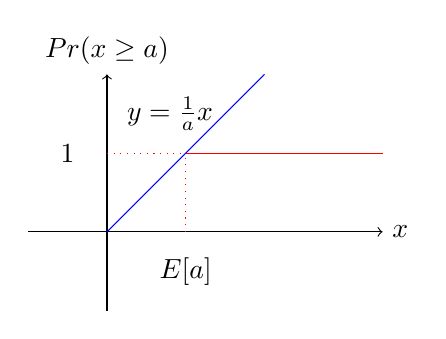
\begin{tikzpicture}
          \draw[->] (-1,0) -- (3.5,0) node[right] {$x$};
          \draw[->] (0,-1) -- (0,2) node[above] {$Pr(x \geq a)$};
          \draw[scale=1,domain=0:2,smooth,variable=\x,blue] plot ({\x},{\x});
          \draw[scale=1,domain=1:3.5,smooth,variable=\x,red] plot ({\x},{1});
          \draw (0.8,1.5) node {$y = \frac{1}{a} x$};
          \draw[scale=1,domain=0:1,dotted,variable=\x,red] plot ({1},{\x});
          \draw (1,-0.5) node {$E[a]$};
          \draw[scale=1,domain=0:1,dotted,variable=\y,red] plot ({\y},{1});
          \draw (-0.5,1) node {$1$};
        \end{tikzpicture}
        \caption{Markov inequality.}
    \end{figure}
    
\end{itemize}

\newpage

\subsection{Chebyshev Bound:}

Generalized version of the Markov bound

\begin{equation*}
    Pr(|X| \geq a) = \int \mathbb{I}_{{|x| \geq a}} f(x) dx \leq \frac{E[X^2]}{a^2}
\end{equation*}

\begin{figure}[ht]
\centering
    \begin{tikzpicture}
      \draw[->] (-3,0) -- (3,0) node[right] {$x$};
      \draw[->] (0,-0.5) -- (0,3) node[above] {$Pr(|x| \geq a)$};
      \draw[scale=1,domain=-1.5:1.5,smooth,variable=\x,blue] plot ({\x},{\x * \x});
      \draw[scale=1,domain=1:3.5,smooth,variable=\x,red] plot ({\x},{1});
      \draw[scale=1,domain=-1:-3.5,smooth,variable=\x,red] plot ({\x},{1});
      \draw[scale=1,domain=0:1,dotted,variable=\x,red] plot ({1},{\x});
      \draw (1,-0.5) node {$a$};
      \draw[scale=1,domain=0:1,dotted,variable=\x,red] plot ({-1},{\x});
      \draw (-1,-0.5) node {$-a$};
      \draw[scale=1,domain=-1:1,dotted,variable=\y,red] plot ({\y},{1});
      \draw (-0.3,1.3) node {$1$};
    \end{tikzpicture}
    \caption{Chebyshev inequality.}
\end{figure}

\subsection{Cantelli's Inequality:}

\begin{itemize}
    
    \item $Pr(x - \mu \geq a)$ using a quadratic function: $h(y) = (y + b)^2$
    
    \begin{figure}[ht]
    \centering
        \begin{tikzpicture}
          \draw[->] (-3,0) -- (3,0) node[right] {$x$};
          \draw[->] (0,-0.5) -- (0,3) node[above] {$Pr(|x| \geq a)$};
          \draw[scale=1,domain=-1:2,smooth,variable=\x,blue] plot ({\x},{(\x - 0.5)^2});
          \draw[scale=1,domain=1.5:3.5,smooth,variable=\x,red] plot ({\x},{1});
          \draw[scale=1,domain=-0.5:-3.5,smooth,variable=\x,red] plot ({\x},{1});
          \draw[scale=1,domain=0:1,dotted,variable=\x,red] plot ({1.5},{\x});
          \draw (1,-0.5) node {$a + \mu$};
          \draw[scale=1,domain=0:1,dotted,variable=\x,red] plot ({-1.5},{\x});
          \draw (-1,-0.5) node {$-a + \mu$};
          \draw[scale=1,domain=-1.5:1.5,dotted,variable=\y,red] plot ({\y},{1});
          \draw (-0.3,1.3) node {$1$};
        \end{tikzpicture}
        \caption{Cantelli's inequality.}
    \end{figure}
    
    \item Shifted quadratic: $\Tilde{h}(y) = \frac{(y + b)^2}{(a + \mu + b)^2}$
    
    \item Assume for the ease of the problem, assume $\mu = 0$: $\Tilde{h}(y) = \frac{(y + b)^2}{(a + b)^2}$, so that the function is above the corner
    
    \item
    
    \begin{equation*}
        \begin{aligned}
            Pr(Y \geq a) &\leq \frac{E[(Y + b)^2]}{(a + b)^2} \\
            &= \frac{E[Y^2] + 2 b E[Y] + b^2}{(a + b)^2} \\
            &= \frac{\sigma^2 + b^2}{(a + b)^2}, b > 0
        \end{aligned}
    \end{equation*}
    
    \item Family of bounds parameterized by $b$: take the highest bound, $\min_{b>0} \frac{\sigma^2 + b^2}{(a + b)^2}$
    
\end{itemize}

\newpage

\section{Lesson 9 2.11.2020}

\subsection{Foundation of Statistical Inference:}

\begin{itemize}

    \item Use PDF $f(x)$ to infer the output $Y$
    
    \item $f(x)$ is a family of distribution based on parameter $\theta$: $f_\theta(x)$ or $f(x;\theta)$
    
    \item Inference: also known as the reverse problem
    
    \item Inference problem: collection of probability distributions, reveals something about $\theta$
    
    \item $\theta$ can be thought of as the attribute set
    
    \item For instance:
    
    \begin{gather*}
        \begin{cases}
            f_0 \sim N(0, \sigma^2) \\
            f_1 \sim N(1, \sigma^2)
        \end{cases}
    \end{gather*}
    
    One candidate is to pick the bigger one, i.e. the maximum likelihood solution: $\max_{\theta} f_{\theta}(y)$
    
    The solution is: $\argmax_{\theta} f_{\theta}(y)$
    
    \item Engineers usually provide solution, as well as optimization
    
\end{itemize}

\subsection{Likelihood Function:}

\begin{itemize}
    
    \item $L(\theta; y) = f_{\theta}(y)$: $\theta$ fixed, $y$ is the argument
    
    \item Defined pointwise
    
    \item Take the PDF of $\theta$, evaluate at $y$
    
    \item Get 1 if integrating the PDF: normalization
    
    \item Think $y$ as fixed, $\theta$ as the parameter
    
    \item Example:
    
    Suppose the parameter space is finite and under the classical setting:
    
    \begin{equation*}
        f_n(y), \theta = 1..n
    \end{equation*}
    
    One possible objective function:
    
    \begin{equation*}
        \max f_n(y)
    \end{equation*}
    
    The solution will be:
    
    \begin{equation*}
        \argmax_{n} f_n(y) = \hat{\theta}_{ML}
    \end{equation*}
    
    \item View the attribute set as probability set: $P(\theta)$ or the PMF, if finite number of $\theta$s
    
    \item Collective goal: produce $\hat{\theta}(y)$ estimator: a function that $\hat{\theta}: y \rightarrow \Theta$
    
    \item Reasonable objective function to evaluate $\hat{\theta}$: $\max f_{\theta}(y) Pr(\theta)$
    
    Answer: i.e. in the discrete case
    
    \begin{equation*}
        \argmax_{\theta} f_{\theta} f_{\theta}(y) Pr(\theta) = \hat{\theta}_{MAP}
    \end{equation*}
    
    Detour:
    
    \begin{equation*}
        \begin{aligned}
            Pr(\theta|y) &= \frac{Pr(\theta \cap \{Y = y\})}{Pr(Y = y)} \\
            &\propto Pr(\theta \cap \{Y = y\}) \text{, directly proportional} \\
            &= f(y|\theta) Pr(\theta) \\
            &= f_{\theta}(y) Pr(\theta)
        \end{aligned}
    \end{equation*}
    
    If $Pr(\theta) = \frac{1}{n}$, then:
    
    \begin{equation*}
        \begin{aligned}
            \argmax_{\theta} f_{\theta}(y) Pr(\theta) &= \argmax_{\theta} f_{\theta}(y) \frac{1}{n} \\
            &= \argmax_{\theta} f_{\theta}(y)
        \end{aligned}
    \end{equation*}
    
    It is a maximum likelihood condition, even under a Bayesian setting.
    
    \item What if $\theta$ is in a continuous space: $\theta$ uncountable but smooth
    
    Objective function: $\max f_{\theta}(y)$
    
    Solution: $\argmax_{\theta} f_{\theta}(y) = \hat{\theta}_{ML}$
    
    Or for MAP: $\argmax_{\theta} f_{\theta}(y) f(\theta)$
    
\end{itemize}

\subsection{Criterion:}

\begin{itemize}
    
    \item A norm squared, the mean square error: MSE
    
    \begin{equation*}
        ||\hat{\theta}(y) - \theta(y)||_2^2 = E[(\hat{\theta}(y) - \theta(y))^2]
    \end{equation*}
    
    \item Find a $\hat{\theta}(y)$ that minimizes mean square error: minimum mean square error, MMSE
    
    \item Overall: optimization applied to specific fields
    
    \item For a difficult problem:
    
    \begin{itemize}
        
        \item Constrain the solution space, i.e. a certain type of function, instead of all possible solution, i.e. the linear function space
        
        \item LMMSE instead of MMSE: L for linear
        
        \item To make the problem solvable
        
    \end{itemize}
    
    \item Constraint: some knowledge about the solution $\rightarrow$ becomes a constrained optimization problem, i.e.
    
    \begin{equation*}
        \begin{aligned}
            Y &= AX + N \\
            Y &= A \theta + N \text{, $X$ plays the role of $\theta$}
        \end{aligned}
    \end{equation*}
    
    Want to produce:
    
    \begin{equation*}
        \hat{\Theta}(y) = \argmin_{\hat{\theta}} E[(\hat{\theta} - \theta)^2]
    \end{equation*}
    
    What if $\theta$ is sparse, i.e.:
    
    \begin{equation*}
        ||\hat{\theta(y)}||_{0} = k
    \end{equation*}
    
\end{itemize}

\subsection{Log Likelihood:}

\begin{itemize}
    
    \item Sometimes the observation is a vector: $\Bar{y} = (y_1...y_m)$, from $\theta$ (one $\theta$), same for all the observation:
    
    \begin{equation*}
        \begin{aligned}
            f_{\theta}(y_1...y_m) &= \prod_{i = 1}^{m} f_{\theta}(y_i) \text{, conditional independent} \\
            L(\Bar{y}; \theta) &= f_{\theta}(y_1...y_m) \\
            &= \prod_{i = 1}^{m}f_{\theta}(y_i) \\
            &= \prod_{i = 1}^{m} L(y_i; \theta) \text{, based on a scalar value instead of vector} \text{, apply $\log$} \\
            \frac{1}{m} \log L(\Bar{y}; \theta) &= \frac{1}{m} \sum_{i = 1}^{m} \log L(y_i; \theta) \\
            &= \frac{1}{m} \sum_{i = 1}^{m} log L(y_i; \theta)
        \end{aligned}
    \end{equation*}
    
    LLN, normalized sum of i.i.d. random variables
    
\end{itemize}

\newpage

\section{Lesson 10 2.13.2020}

\subsection{Principle of Data Reduction:}

\begin{itemize}
    
    \item $X$: observation, say something about $\theta$
    
    \item A sequence of observation: $x_1, x_2...x_n = \Bar{X}$
    
    \item $T(\Bar{X}), X^n \rightarrow \mathbb{R}$: a statistic, a realization of the data, functions
    
    \item Example:
    
    \begin{equation*}
        \begin{aligned}
            T_1(\Bar{X}) &= \frac{1}{n} \sum_{i = 1}^{n} x_i \text{, the empirical mean} \\
            T_2(\Bar{X}) &= \frac{1}{n - 1} \sum_{i = 1}^{n} (x_i - \Bar{X})^2 \text{, the empirical variance} \\
            T_3(\Bar{X}) &= \max_{i = 1..n} x_i \\
            T_4(\Bar{X}) &= \min_{i = 1..n} x_i
        \end{aligned}
    \end{equation*}
    
    \item Need to reduce data in many cases
    
    \item Example:
    
    Vote for one of the two candidates:
    
    \begin{gather*}
        B = 
        \begin{cases}
        1 \text{, with probability $\theta$} \\
        0\text{, with probability $1-\theta$} \\
        \end{cases}
    \end{gather*}
    
    Poll result: $(w...w) \rightarrow$ a really long vector that can come up with a prediction for $\theta$. Do I need to carry the vector around? Can I reduce the vast amount of data without losing "information" in a statistical sense and performance? i.e. $T: {0, 1}^10000 \rightarrow \mathbb{N}$
    
    \begin{equation*}
        T: {0, 1}^{10000} \rightarrow \mathbb{R} \text{, } T(\Bar{B}) = \frac{||b||_1}{10000}
    \end{equation*}
    
    \item $X...\rightarrow \theta$: $X$ gives some information about $\theta$
    
    \item $X...\rightarrow T(X) ... \rightarrow\theta$: reduce $X$ using $T(.)$, then give some information about $\theta$, without losing "information"
    
\end{itemize}

\subsection{The Likelihood Function:}

\begin{itemize}
    
    \item $L(\theta, \Bar{X}) = f_{\theta}(\Bar{X})$: know the relation between $\theta$ and $\Bar{X}$
    
    \item Use the notion of conditional probability:
    
    \begin{equation*}
        \begin{aligned}
            P_{\theta}(\Bar{X} = x, T(\Bar{X}) = t) &= P_{\theta}(\Bar{X} = \Bar{x} | T(\Bar{X}) = t)P_{\theta}(T(\Bar{X}) = t) \\
            &= P_{\theta}(T(\Bar{X}) = t | \Bar{X} = \Bar{x})P_{\theta}(\Bar{X} = \Bar{x})
        \end{aligned}
    \end{equation*}
    
    ``All the information is in $T(.)$''
    
    \item Therefore $P_{\Bar{X} = \Bar{x}}(X=x|T(X) = t)$ cannot be a function of $\theta$ in order for it not to contain any information or vary with $\theta$ and for sufficient statistic
    
    \item $\Bar{b} = (b_1, b_2...b_n)$: outcome of a poll
    
    \item $L(\theta; \Bar{b}) = \theta^(b_1)(1-\theta)^{1-b_1}$: likelihood of a certain $\theta$
    
    \item $\Bar{b}$ fixed, varying $\theta$, see how it varies:
    
    \begin{equation*}
        \begin{aligned}
            \prod_{i = 1}^{n}\theta^{b_i}(1 - \theta)^{1 - b_i} &= \theta^{\sum_{i = 1}^{n} b_i}(1 - \theta)^{n - \sum_{i = 1}^{n} b_i} \\ 
            &= \theta^{T(\Bar{b})}(1-\theta)^{n - T(\Bar{b})}
        \end{aligned}
    \end{equation*}
    
    \item $P_{\theta}(\Bar{B} = \Bar{b} | T(\Bar{B}) = t) P_{\theta}(T(\Bar{B}) = t)$:
    
    \begin{gather*}
        \begin{cases}
            P_{\theta}(\Bar{B} = \Bar{b} | T(\Bar{B}) = t) \rightarrow \text{the residual} \frac{1}{{n \choose t}} \\
            P_{\theta}(T(\Bar{B}) = t) \rightarrow \theta^{T(\Bar{b})}(1-\theta)^{n - T(\Bar{b})}
        \end{cases}
    \end{gather*}
    
    \item The residual: $\mathbb{I}_{\{t = ||\Bar{b}||_0\}}$
    
    \begin{equation*}
        \frac{P_{\theta}(\Bar{B} = \Bar{b} \cap T(\Bar{B}) = t)}{P_{\theta}(T(\Bar{B}) = t)} = \frac{\theta^{t}(1 - \theta)^{n - t}}{{n \choose t} \theta^{t}(1 - \theta)^{n - t}} = \frac{1}{{n \choose t}}
    \end{equation*}
    
    This means if they match, what is the probability of a certain pattern
    
\end{itemize}

\subsection{Sufficient Statistic:}

\begin{itemize}
    
    \item A statistic $T(\Bar{x})$ is sufficient for $\theta$ if the conditional distribution of $X$ given $T(X)$ does not depend on $\theta$
    
    \begin{equation*}
        \begin{aligned}
            P_{\theta}(\Bar{X} = \Bar{x} | T(\Bar{X}) = T(\Bar{x})) &= \frac{P_{\theta}(\Bar{X} = \Bar{x}, T(\Bar{X}) = T(\Bar{x}))}{P_{\theta}(T(\Bar{X}) = T(\Bar{x}))} \\
            &= \frac{P_{\theta}(\Bar{X} = \Bar{x})}{P_{\theta}(T(X) = T(x))}
        \end{aligned}
    \end{equation*}
    
    If all the information is in $T(X)$, then the ratio should not depend on $\theta$
    
\end{itemize}

\subsection{Factorization Theorem:}

\begin{itemize}
    
    \item $f(x|\theta)$: distribution of $X$ under $\theta$
    
    \item $T(X)$ is a sufficient statistic for $\theta$ if and only if there exists $g(t|\theta)$ and $h(x)$ such that all $X$'s and all $\theta$s:
    
    \begin{equation*}
        f(x|\theta) = g(T(x)|\theta)h(x)
    \end{equation*}
    
    i.e. a parameterized distribution
    
    \item Proof:
    
    Suppose $T(X)$ is a sufficient statistic:
    
    \begin{equation*}
        \begin{aligned}
            f(x|\theta) &= P_{\theta}(X = x) \text{, if true} \\
            &= P_{\theta}(X = x, T(X) = T(\Bar{x}))
        \end{aligned}
    \end{equation*}
    
    Introduce the conditional version:
    
    \begin{gather*}
        \begin{cases}
            P_{\theta}(X = x | T(X) = T(\Bar{x})) \rightarrow h(\Bar{x}) \text{, function of the residual, independent of }\theta \\
            P_{\theta}(T(X) = T(\Bar{x})) \rightarrow g(T(x)|\theta)
        \end{cases}
    \end{gather*}
    
    How about the reverse side? Since we are trying to prove an if-and-only-if hypothesis:
    
    Assume the factorization exists:
    
    \begin{equation*}
        f(x|\theta) = g(T(x)|\theta)h(x)
    \end{equation*}
    
    Aiming for a particular mapping:
    
    \begin{equation*}
        \frac{f(x|y)}{P_{\theta}(T(X) = T(x))}
    \end{equation*}
    
    Want the ratio to be constant independent of $\theta$:
    
    \begin{equation*}
        \begin{aligned}
            \frac{g(T(x)|\theta)h(\Bar{x})}{P_{\theta}(T(X) = T(x))} \\
            P_{\theta}(T(X) = T(x)) &= P_{\theta}(T(X) = t) \\
            &= P_{\theta}(x = T^{-1}(t)) \text{, the pre-image} \\
            &= \sum_{x \in T^{-1}(t)} f(x|\theta) \\
            &= \sum_{x \in T^{-1}(t)} g(T(x)|\theta) h(x) \\
            \frac{g(T(x)|\theta)h(\Bar{x})}{P_{\theta}(T(X) = T(x))} &= \frac{g(T(x)|\theta)h(\Bar{x})}{\sum_{x \in T^{-1}(t)} g(T(x)|\theta) h(x)} \\
            &= \frac{h(\Bar{x})}{\sum_{x \in T^{-1}(t)} h(x)} \rightarrow \text{independent of } \theta
        \end{aligned}
    \end{equation*}
    
\end{itemize}

\end{document}
